\documentclass[11pt,compress,t,notes=noshow, aspectratio=169, xcolor=table]{beamer}

\usepackage{../../style/lmu-lecture}
% Defines macros and environments
\input{../../style/common.tex}

\title{Applied Machine Learning}
% \author{LMU}
%\institute{\href{https://compstat-lmu.github.io/lecture_iml/}{compstat-lmu.github.io/lecture\_iml}}
\date{}

\begin{document}

\newcommand{\titlefigure}{figure/performance_vs_interpretability}
\newcommand{\learninggoals}{
\item The Hyperparameter Optimization Problem
\item Grid Search, Random Search and Bayesian optimization
\item The Untouched Test Set Principle}

\lecturechapter{Applied Hyperparameter Tuning}
\lecture{Applied Machine Learning}


\section{Hyperparameter Tuning}

\begin{frame}{}
    \includepdf[pages={2},trim=0 20 0 0,clip,width=490pt,offset=20pt 0pt,pagecommand={}]{i2ml/slides-tuning-intro.pdf}
\end{frame}

\begin{frame}{}
    \includepdf[pages={3},trim=0 20 0 0,clip,width=490pt,offset=20pt 0pt,pagecommand={}]{i2ml/slides-tuning-intro.pdf}
\end{frame}

\begin{frame}{}
    \includepdf[pages={4},trim=0 20 0 0,clip,width=490pt,offset=20pt 0pt,pagecommand={}]{i2ml/slides-tuning-intro.pdf}
\end{frame}

\begin{frame}{}
    \includepdf[pages={5},trim=0 20 0 0,clip,width=490pt,offset=20pt 0pt,pagecommand={}]{i2ml/slides-tuning-intro.pdf}
\end{frame}

\begin{frame}{}
    \includepdf[pages={6},trim=0 20 0 0,clip,width=490pt,offset=20pt 0pt,pagecommand={}]{i2ml/slides-tuning-intro.pdf}
\end{frame}

\begin{frame}{}
    \includepdf[pages={7},trim=0 20 0 0,clip,width=490pt,offset=20pt 0pt,pagecommand={}]{i2ml/slides-tuning-intro.pdf}
\end{frame}

\begin{frame}{}
    \includepdf[pages={8},trim=0 20 0 0,clip,width=490pt,offset=20pt 0pt,pagecommand={}]{i2ml/slides-tuning-intro.pdf}
\end{frame}

\begin{frame}{}
    \includepdf[pages={9},trim=0 20 0 0,clip,width=490pt,offset=20pt 0pt,pagecommand={}]{i2ml/slides-tuning-intro.pdf}
\end{frame}

\section{Hyperparameter Tuning Algorithms}

\begin{frame}{}
    \includepdf[pages={2},trim=0 20 0 0,clip,width=490pt,offset=20pt 0pt,pagecommand={}]{i2ml/slides-tuning-basicalgos.pdf}
\end{frame}

\begin{frame}{}
    \includepdf[pages={4},trim=0 20 0 0,clip,width=490pt,offset=20pt 0pt,pagecommand={}]{i2ml/slides-tuning-basicalgos.pdf}
\end{frame}

\begin{frame}{}
    \includepdf[pages={6},trim=0 20 0 0,clip,width=490pt,offset=20pt 0pt,pagecommand={}]{i2ml/slides-tuning-basicalgos.pdf}
\end{frame}

\begin{frame}{}
    \includepdf[pages={7},trim=0 20 0 0,clip,width=490pt,offset=20pt 0pt,pagecommand={}]{i2ml/slides-tuning-basicalgos.pdf}
\end{frame}

\begin{frame}{Summary}
    \begin{table}[]
        \centering
        \begin{tabular}{l|cc}
            Property & Grid Search & Random Search \\
            \midrule
            Easy to implement & $\checkmark$ & $\checkmark$ \\
            All parameter types possible & $\checkmark$ & $\checkmark$ \\
            Parallelization is trivial & & $\checkmark$ \\
            Does not suffer from the curse of dimensionality & & $\checkmark$ \\
            Does not require discretization of hyperparameters & & $\checkmark$ \\
            Anytime algorithm & & $\checkmark$
        \end{tabular}
    \end{table}
\end{frame}

\section{The Untouched Test Set Principle}
\begin{frame}{The Untouched Test Set Principle}

\begin{itemize}
\setlength\itemsep{2em}
    \item 
\end{itemize}
\end{frame}

\begin{frame}{Train-Valid-Test Protocol}

\begin{itemize}
\setlength\itemsep{2em}
    \item 
\end{itemize}
\end{frame}

\begin{frame}{Nested Cross-Validation}

\begin{itemize}
\setlength\itemsep{2em}
    \item 
\end{itemize}
\end{frame}

\begin{frame}{Most important factor in ML: correct CV}

\begin{itemize}
\setlength\itemsep{2em}
    \item 
\end{itemize}
\end{frame}

\section{Pipelines}
\begin{frame}{Learn operations only on the training set}

\begin{itemize}
\setlength\itemsep{2em}
    \item 
\end{itemize}
\end{frame}

\endlecture
\end{document}
